\documentclass[aspectratio=169]{beamer}
\usetheme{metropolis}
\metroset{block=fill}
\usepackage{tikz}
\usetikzlibrary{positioning, arrows.meta, shapes.geometric}

\title{Building a Reproducible Scholarly Search Toolkit}
\subtitle{Episode 0: Why Build This?}
\author{Scholar Search Kit}
\date{}

\begin{document}

\begin{frame}[plain]
  \titlepage
\end{frame}

\begin{frame}{The Scientific Need}
  \begin{itemize}
    \item \textbf{Exploratory Research} often relies on proprietary algorithms.
    \item \textbf{Systematic Literature Reviews (SLR)} demand absolute transparency.
    \item \textbf{The Core Problem}: Most tools inextricably couple \textit{search mechanics} with the \textit{research methodology}.
  \end{itemize}
\end{frame}

\begin{frame}{The Goal of this Toolkit}
  \begin{itemize}
    \item Build a \textbf{modular}, \textbf{extensible}, and \textbf{scientifically auditable} search toolkit.
    \item Support multiple providers through a unified interface.
    \item Decouple the execution of search and deduplication from the theoretical research protocol.
  \end{itemize}
  
  \vspace{0.5cm}
  \begin{center}
  \resizebox{\linewidth}{!}{
  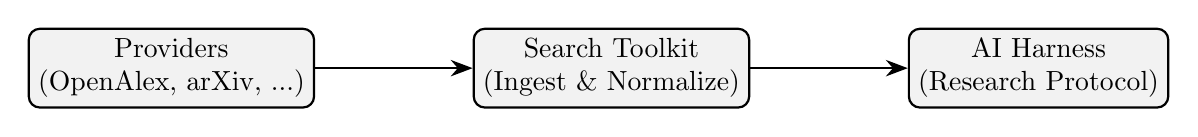
\begin{tikzpicture}[
      node distance=1.5cm and 2cm,
      box/.style={rectangle, draw, thick, rounded corners, align=center, minimum width=2.5cm, minimum height=1cm, fill=black!5},
      arrow/.style={-{Stealth[scale=1.2]}, thick}
    ]
    \node[box] (providers) {Providers\\(OpenAlex, arXiv, ...)};
    \node[box, right=of providers] (toolkit) {Search Toolkit\\(Ingest \& Normalize)};
    \node[box, right=of toolkit] (harness) {AI Harness\\(Research Protocol)};

    \draw[arrow] (providers) -- (toolkit);
    \draw[arrow] (toolkit) -- (harness);
  \end{tikzpicture}
  }
  \end{center}
\end{frame}

\begin{frame}{Why Build from Scratch?}
  \begin{alertblock}{Auditability over Convenience}
    We cannot scientifically trust what we cannot trace. By building from first principles, we guarantee the provenance of every deduplicated record and every normalized timestamp.
  \end{alertblock}
  \vspace{0.5cm}
  \begin{itemize}
    \item We learn \textbf{resilient design} (rate limiters, token buckets).
    \item We understand \textbf{API discrepancies} across providers.
    \item We prepare for \textbf{AI orchestration} (building CLI tools that an AI agent can reliably execute).
  \end{itemize}
\end{frame}

\begin{frame}{What to Expect}
  \begin{enumerate}
    \item \textbf{Season 1}: Foundation \& Contracts
    \item \textbf{Season 2}: Data Models \& Resilience
    \item \textbf{Season 3}: Providers \& Ingestion
    \item \textbf{Season 4}: Matching \& Export
    \item \textbf{Season 5}: CLI, Harness \& AI
  \end{enumerate}
\end{frame}

\begin{frame}[standout]
  Let's start reading the contract!
\end{frame}

\end{document}
